%!TEX program = xelatex
\documentclass[10pt]{article}
\usepackage{amssymb}
\usepackage{amsmath}
\usepackage{mathrsfs}
\usepackage{titlesec}
\usepackage{xcolor}
%\usepackage[shortlabels]{enumitem}
\usepackage{enumerate}
\usepackage{bm}
\usepackage{tikz}
\usepackage{listings}
\usetikzlibrary{arrows}
%\usepackage{subfigure}
\usepackage{graphicx,booktabs,multirow}
\usepackage[a4paper]{geometry}
\usepackage{upquote}
\usepackage{float}
\usepackage{pdfpages}

\usepackage[colorlinks,linkcolor=blue]{hyperref}
\usepackage{mdframed}

\usepackage{caption}
\graphicspath{{images/}}
\usepackage{subfig}

\iffalse
\usepackage{lastpage}
\usepackage{fancyhdr}
\fancyfoot[C]{Page \thepage\ of \pageref{LastPage}}
% Uncomment to remove the header rule
\renewcommand{\headrulewidth}{0pt} 
\pagestyle{fancy}
\fi

\geometry{verbose,tmargin=2cm,bmargin=2cm,lmargin=2cm,rmargin=2cm}
\geometry{verbose,tmargin=2cm,bmargin=2cm,lmargin=2cm,rmargin=2cm}
\lstset{language=Matlab}
\lstset{breaklines}

\input defs.tex

\newenvironment{solution}
    { \begin{mdframed}[backgroundcolor=gray!10] \textcolor{cyan}{\textbf{Solution}} \\}
    {  \end{mdframed}}

\newtheorem{proposition}{Proposition}
\newtheorem{remark}{Remark}

\titleformat*{\section}{\centering\LARGE\scshape}
\renewcommand{\thesection}{\Roman{section}}
\lstset{language=Matlab,tabsize=4,frame=shadowbox,basicstyle=\footnotesize,
keywordstyle=\color{blue!90}\bfseries,breaklines=true,commentstyle=\color[RGB]{50,50,50},stringstyle=\ttfamily,numbers=left,numberstyle=\tiny,
  numberstyle={\color[RGB]{192,92,92}\tiny},backgroundcolor=\color[RGB]{245,245,244},inputpath=code}

\begin{document}

\title{CS150: Database and Data Mining \\%
	Final Exam Solutions}
\maketitle


\section{Basics \textbf{[10 points]}}
For each image on the next page, select the letter corresponding to the best description. \\
A. Left Deep Tree \\
B. Key Compression \\
C. B+ Tree \\
D. Spark \\
E. Nested Loops Join \\
F. Sort Merge Join \\
G. Page Nested Loop Join \\
H. Slotted Page \\
I. Variable Length Tuple \\
J. Fixed Length Tuple \\
K. Buffer Frame \\
L. Sort-based Group-by \\
M. Recovery \\
N. Two Phase Lock \\
O. JSON \\
P. ISAM \\
Q. External Sort \\
R. MapReduce
\begin{solution}
	1. Q  \\
	2. A  \\
	3. M  \\
	4. R  \\
	5. N \\
	6. H  \\
	7. O  \\
	8. C \\
	9. D  \\
	10. G  \\
\end{solution}
%\newpage
\begin{figure}
	\centering
	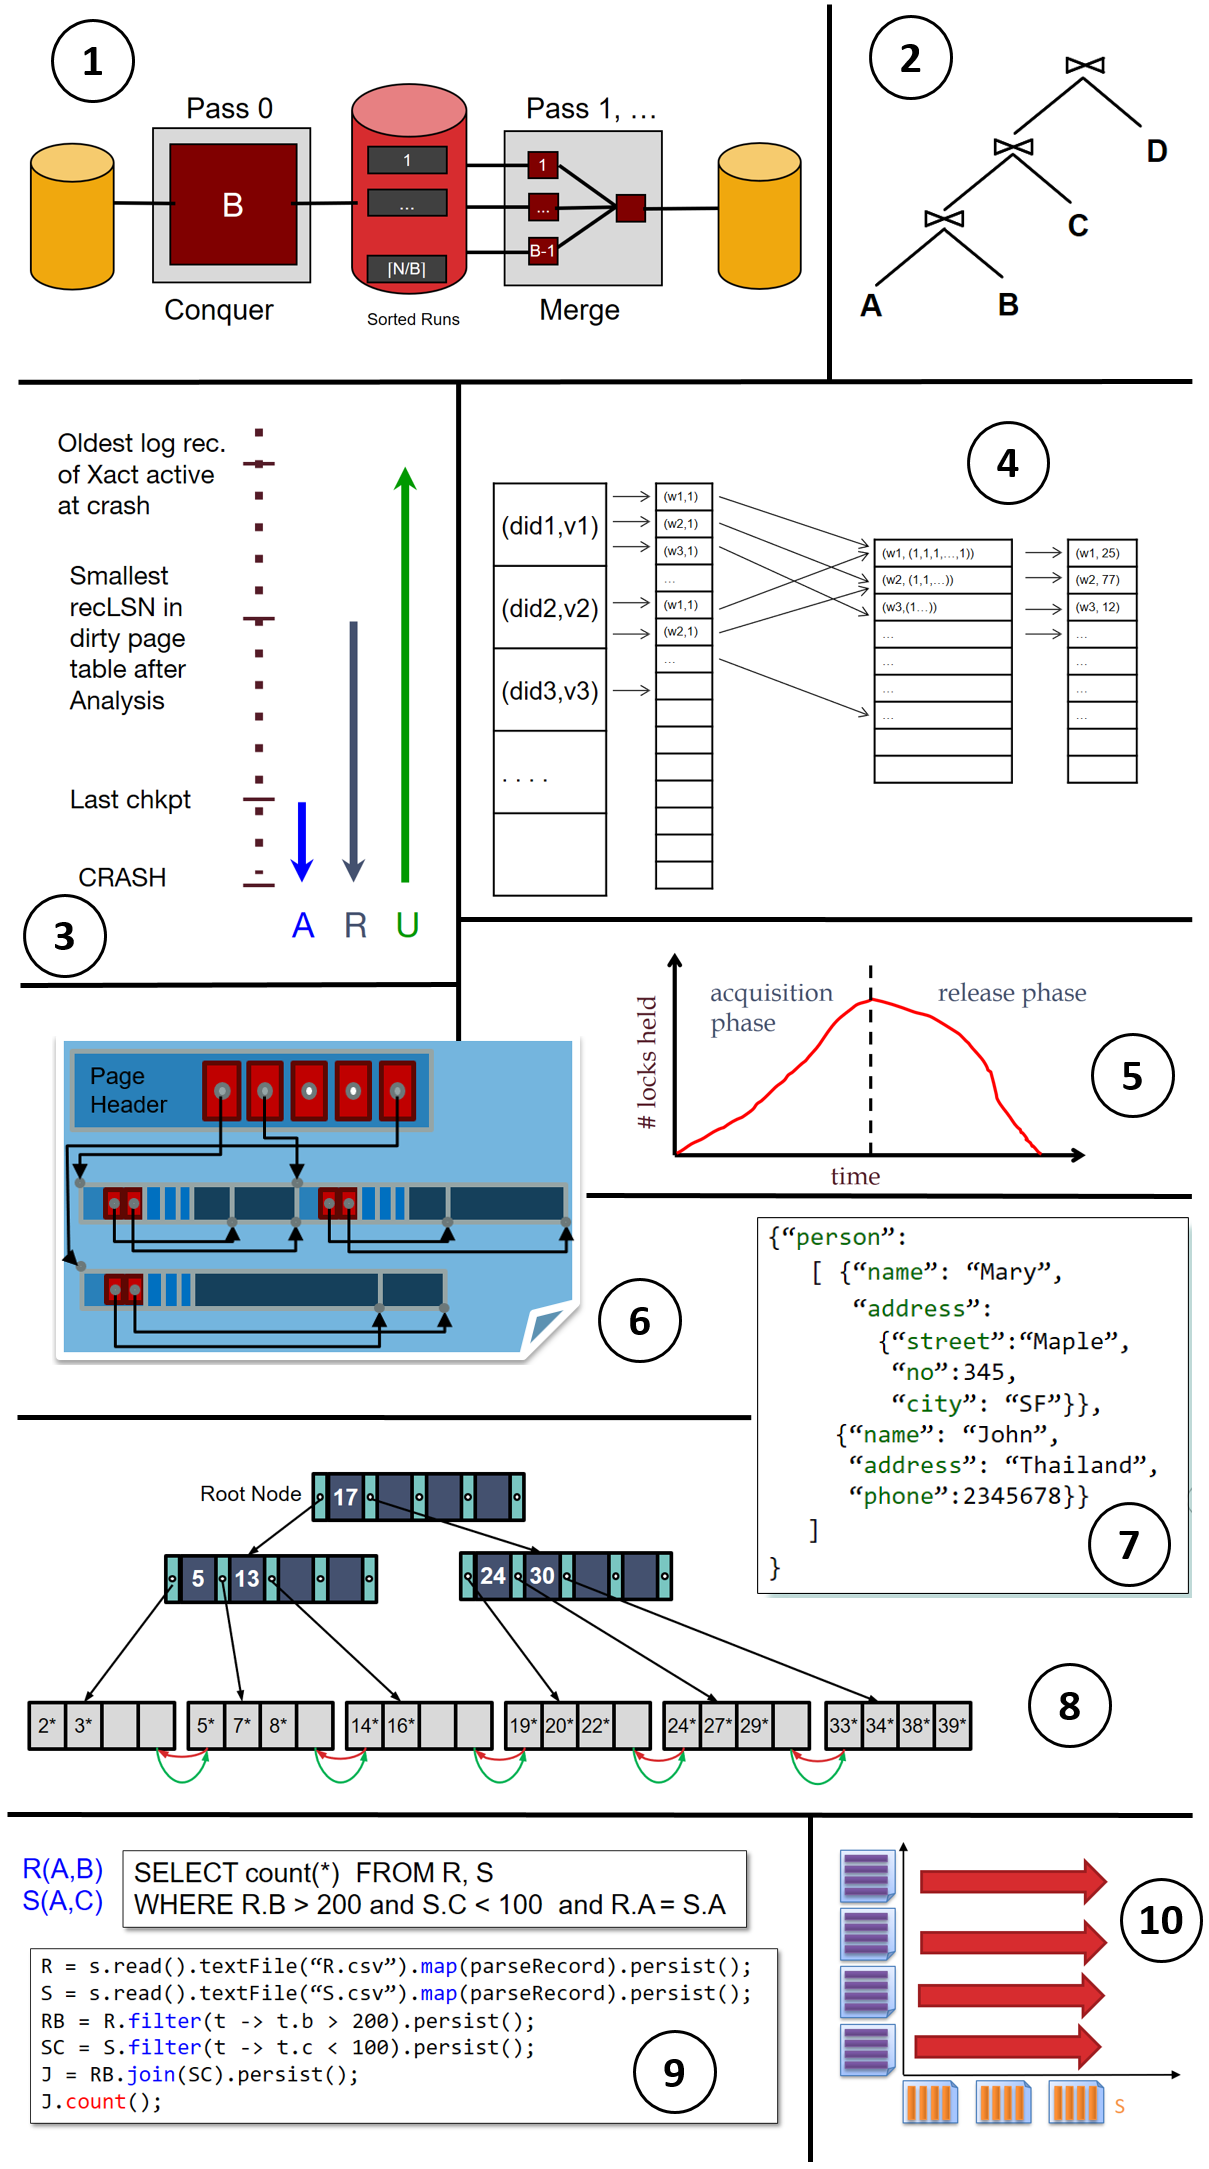
\includegraphics[width=.8\linewidth]{basics_new.png}
\end{figure}


\newpage
\section{SQL \textbf{[12 points]}}
\begin{enumerate}

	\item \textbf{[2 points]}
	      Which of the following expressions computes the matrix vector product:
	      $$
		      (\mathbf{A} \mathbf{x})_{i}=\sum_{k=1}^{d} A_{i k} x_{k}
	      $$
	      Assume $\mathbf{A}$ and $\mathbf{x}$ have compatible dimensions and there is only one correct answer.\\
	      A.

	      \begin{lstlisting} 
SELECT A.row AS row, SUM(A.value * x.value) AS value 
FROM A JOIN x
ON A.col = x.row
GROUP BY A.row
\end{lstlisting}


	      B.
	      \begin{lstlisting}
SELECT A.row AS row, SUM(A.value * x.value) AS value 
FROM A JOIN x
ON A.row = x.row
GROUP BY A.col
\end{lstlisting}
	      C.
	      \begin{lstlisting} 
SELECT x.row AS row, SUM(A.value * x.value) AS value 
FROM A JOIN x
ON A.col = x.row
GROUP BY A.col
\end{lstlisting}
	      D.
	      \begin{lstlisting}
SELECT A.row AS row, A.value * x.value AS value 
FROM A JOIN x
ON A.row = x.row
\end{lstlisting}

	      \begin{solution}
		      A: The final answer should be grouped by the row of A and therefore sum over the product along the columns.
	      \end{solution}



	\item \textbf{[2 points]}
	      Suppose we wanted to compute the element-wise sum of the vectors $\mathbf{x}$
	      and $\mathbf{y}$ using the SQL expression:
	      \begin{lstlisting}
SELECT x.row AS row, SUM(x.value + y.value) AS value 
FROM x JOIN y 
ON x.row = y.row
\end{lstlisting}
	      Which of the following statements about this query are true?
	      (You may mark zero ($\phi$), one or more than one of the choices.)\\
	      A. Some non-zero entries may be omitted from the final result.\\
	      B. The correct query should use LEFT OUTER JOIN.\\
	      C. The correct query should use FULL OUTER JOIN.\\
	      D. There is nothing wrong.
	      \begin{solution}
		      A, C: There was a typo in this question (sum should be removed).
		      The issue with this query is the combination of two factors.
		      First, the two vectors may have zeros in different places,
		      and in a sparse vector the zero entries are represented by
		      the absence of information (missing row IDs in the table).
		      Second, by default, joins in SQL will discard a tuple from one
		      table unless it has a match in the other table; OUTER JOINs
		      preserve these non-matching tuples. \\
		      Consider the following:
		      \begin{center}
			      \begin{tabular}{|l|l|}
				      \multicolumn{2}{c} {Vector a} \\
				      \hline Row & Value            \\
				      \hline 1   & 3.0              \\
				      \hline 3   & 4.0              \\
				      \hline
			      \end{tabular} \qquad \qquad
			      \begin{tabular}{|l|l|}
				      \multicolumn{2}{c} {Vector b} \\
				      \hline Row & Value            \\
				      \hline 2   & 2.0              \\
				      \hline 5   & 8.0              \\
				      \hline
			      \end{tabular}
		      \end{center}
		      These two tables produce no outputs on a typical (inner) join,
		      representing a vector of all 0’s.  We need to do a full outer join
		      to ensure that we get rows 1, 2, 3 and 5 in the output.
	      \end{solution}

	
\end{enumerate}


\newpage
\section{Indexes and B+ Trees \textbf{[9 points]}}

\begin{enumerate}

	
	\item \textbf{[4 points]}
	      Consider the following B+ tree of order 2.
	      \begin{center}
		      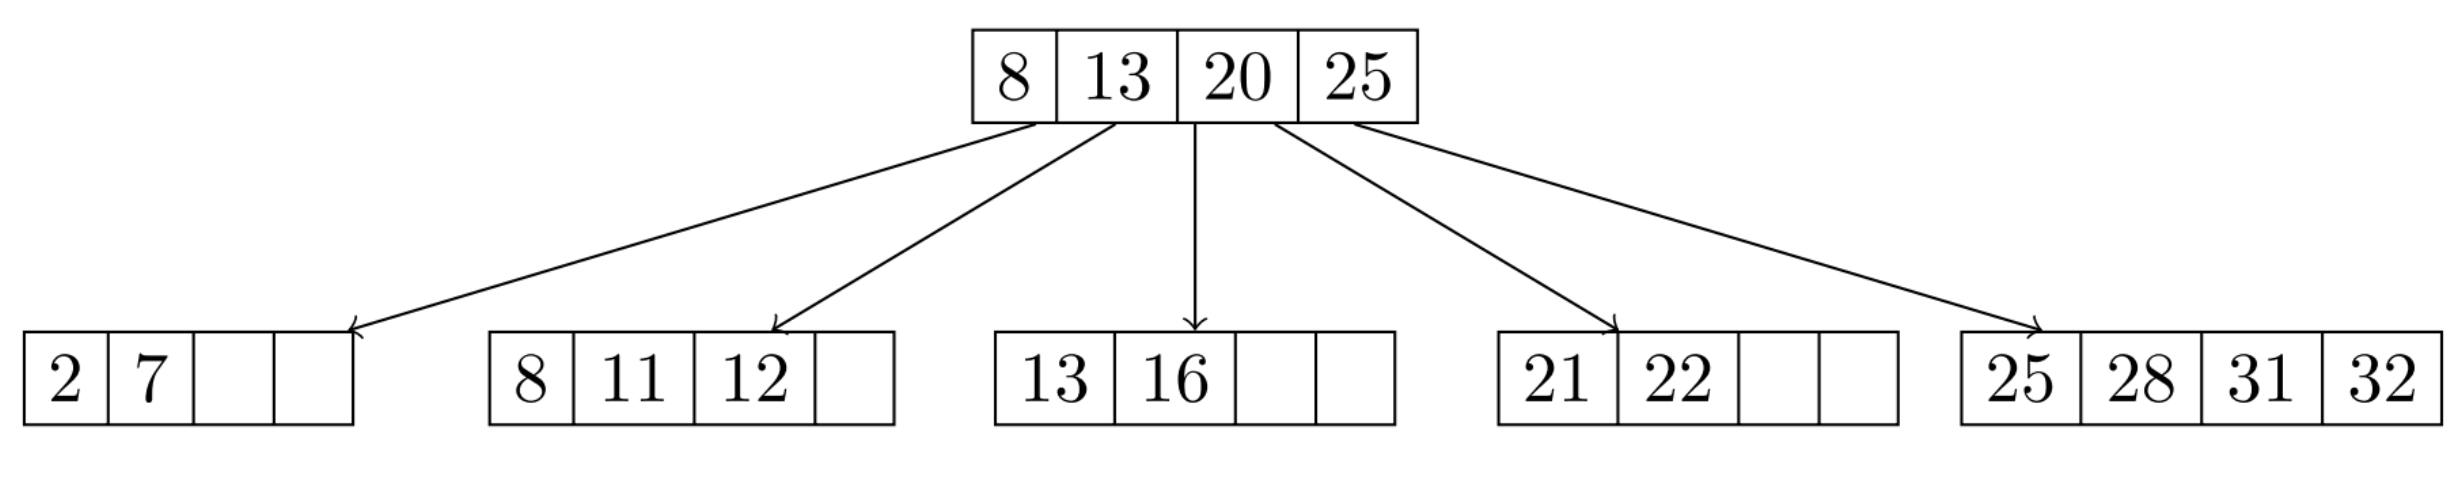
\includegraphics[scale=0.25]{Btree.png}
	      \end{center}
	      \begin{itemize}
		      \item[(a)] \textbf{[1 point]} How many nodes split when you insert 27?
		            \begin{solution}
			            \begin{itemize}
				            \item To insert 27, we follow the rightmost pointer in the tree from the root node because
				                  $27 > 8$, $27 > 13$, $27 > 20$, $27 > 25$.
				            \item We get to the leaf node containing (25, 28, 31, 32) and attempt to insert 27, but the leaf node
				                  is at maximum capacity and the insertion breaks the occupancy invariant. Therefore we must
				                  split the leaf into (25, 27) and (28, 32, 21) and copy up key 27 because this is a leaf node.
				            \item We attempt to insert 27 into the parent node containing (8, 13, 20, 25) but the root is also at
				                  maximum capacity. We split it into (8, 13) and (25, 28) pushing up key 20 because it is an
				                  inner node. Our final tree looks like and we split two nodes.
			            \end{itemize}
		            \end{solution}

		      \item[(b)] \textbf{[1 point]} After inserting 27 into the tree, you also insert 26. How many nodes split as a result of inserting
		            26?
		            \begin{solution}
			            \begin{itemize}
				            \item To insert 26, we first look at the root node and follow the right pointer because 26 $\geq$ 20. We
				                  then follow the middle pointer at the inner node below the root node because $26 > 25$ but
				                  $26 < 28$. We get to the leaf node containing (25, 27)
				            \item We attempt to insert 26 into the leaf node containing (25, 27) and since 3 is less than the
				                  occupancy invariant 4 we insert 26 and are done. We did not split any nodes.
			            \end{itemize}
		            \end{solution}

		      \item[(c)] \textbf{[2 points]} Assume that after inserting 26 and 27, you insert the keys 34, 35, 36, . . ., 100. After all these
		            insertions, what keys are in the leftmost leaf node?
		            \begin{solution}
			            You should be able to identify that we are only inserting keys into the right side of the
			            tree. This is similar to bulk loading in that the left leaf nodes will not be touched. Therefore, we
			            know that the leftmost leaf node will not be modified and will contain (2, 7) after the insertions to
			            the right side of the tree.
		            \end{solution}
	      \end{itemize}
\end{enumerate}




\newpage
\section{B+ Trees and Buffer Management \textbf{[8 points]}}
\begin{enumerate}

	\item \textbf{[6 points]}
	      

	Supposed we have a buffer pool size of 4 pages, and the following access pattern: \\
	A P P L E S A N D B A N A N A S A N D O R A N G E S \\
	Assume that pages are unpinned immediately (ignore pinning).


	      \begin{itemize}
		      \item[(a)] \textbf{[2 points]} What is the number of cache hits if we
			  use an LRU replacement policy? Assume we are starting from a cold (empty) cache.
		            \begin{solution}
			            8
		            \end{solution}
		      \item[(b)] \textbf{[2 points]} What is the number of cache hits if we
			  use an MRU replacement policy? Assume we are starting from a cold (empty) cache
		            \begin{solution}
			            5
		            \end{solution}
		      \item[(c)] \textbf{[2 points]} What is the number of cache hits if we
			  use a CLOCK replacement policy? Assume we are starting from a cold (empty) cache.
		            \begin{solution}
						8
		            \end{solution}
							      \item[(d)] \textbf{[2 points]} What is the number of set reference bits
at the end of (c)?
		            \begin{solution}
						4
		            \end{solution}
	      \end{itemize}
\end{enumerate}



\newpage
\section{External Sorting \textbf{[8 points]}}
\begin{enumerate}

	\item \textbf{[6 points]}
	      Assume that each page is 4 KB large, and that you have a 24KB buffer pool (with 6 frames).
	      \begin{itemize}
		      \item[(a)] \textbf{[2 points]} How many passes would it take to externally sort an 512KB file?
		            Include the initial sorting pass and subsequent merging passes in your answer. You need to simplify your answer.
		            \begin{solution}
			            3: The file contains 128 pages, and B = 6, and thus we need
			            $\left(1+\left\lceil\log _{5}\left(\left\lceil\frac{128}{6}\right\rceil\right)\right\rceil=3\right)$ passes.
		            \end{solution}
		      \item[(b)] \textbf{[2 points]} What would be the total cost in I/Os for this external sort?
		            \begin{solution}
			            768: 2∗128∗$\#$passes = 256*3 = 768 (I/Os).
		            \end{solution}
		      \item[(c)] \textbf{[2 points]} What is the minimum number of additional buffer frames we require to reduce the number of passes
		            (from part 1) by 1?
		            \begin{solution}
			            6: In order to sort the file in two passes, we need B buffer frames
			            where $B(B - 1) \geq 128$. The smallest such B is 12.
			            Thus, the number of additional pages is 12 − 6 = 6.
		            \end{solution}
	      \end{itemize}
\end{enumerate}


\newpage
\section{Join Algorithms \textbf{[8 points]}}

\begin{enumerate}
	\item \textbf{[5 points]}
	      Consider a relation R with attributes $(x,y)$ and a relation S with attributes $(y, z)$.
	      Column $y$ in S is a key and the set of values of $y$ in R are the same as the set of values of $y$ in S.
	      Assume that there are no indexes available and that there are 25 pages in the buffer available.
	      Table R is 1,500 pages with 50 tuples per page. Table S is 400 with 100 tuples per page.
	      Compute the I/O costs for the following joins. Assume the simplest cost model, where pages are read and written one at a time.
	      \begin{itemize}
		      \item[(a)] \textbf{[1 point]} Block nested loops join with R as the outer relation and S as the inner relation.
		            \begin{solution}
			            $|R| + \lceil |R| / B \rceil \times |S| = 1500 + \lceil 1500/25 \rceil \times 400 = 25500$  OR \\
			            $|R| + \lceil |R| / (B-1) \rceil \times |S| = 1500 + \lceil 1500/24 \rceil \times 400 = 26700$ OR \\
			            $|R| + \lceil |R| / (B-2) \rceil \times |S| = 1500 + \lceil 1500/23 \rceil \times 400 = 27900$\\
			            Since, these three equations all appears in some materials, any were acceptable.
		            \end{solution}
		      \item[(b)] \textbf{[1 point]} Sort merge join with S as the outer relation and R as the inner relation.
		            \begin{solution}
			            12500: Same as (c).
		            \end{solution}
		      \item[(c)] \textbf{[1 point]} Hash join with S as the outer relation and R as the inner relation.
		            \begin{solution}
			            5700: $3( \lceil R \rceil + \lceil S \rceil ) = 3(1500 + 400) = 5700$.
		            \end{solution}
	      \end{itemize}

	\item \textbf{[3 points]}
	      Consider a new case, i.e. B>4 pages worth of buffer space, and relations M and N of size > B.
	      Please fill the blanks below with ``always'', ``sometimes'' or ``never''.
	      \begin{itemize}
		      \item[(a)] \textbf{[1 point]} Block nested loop join is \underline{\ \ \ \ \ \ \ \ \ \ } better than page-oriented nested loop join.
		            \begin{solution}
			            Always: Block nested loop join is page-oriented on steroids, and steroids are always good.
		            \end{solution}
		      \item[(b)] \textbf{[1 point]} Sort-merge join is \underline{\ \ \ \ \ \ \ \ \ \ } better than hash-join.
		            \begin{solution}
lo			            Sometimes: Hash join is cooler if one relation is really small and one is very large. Sort dominates if you have lots of duplicate join keys.
		            \end{solution}
		      \item[(c)] \textbf{[1 point]} Hybrid Hash-Join is \underline{\ \ \ \ \ \ \ \ \ \ } better than block-nested loops join.
		            \begin{solution}
			            Sometimes: Nested loops works for non-equijoins and hash does not.
			            For equijoins, hash is often better since it only makes a small number of passes over each relation, whereas block nested- loops still may visit the inner relation many times. If one relation fits in memory, the two algorithms are about equivalent.
		            \end{solution}
	      \end{itemize}
\end{enumerate}



\newpage
\section{Transactions and Concurrency \textbf{[20 points]}}

\begin{enumerate}

	\item \textbf{[4 points]} \textbf{Transactions} \\
	      Consider the following schedule. (For each of the questions below, you may mark zero ($\phi$), one
	      or more than one of the choices.)
	      \begin{center}
		      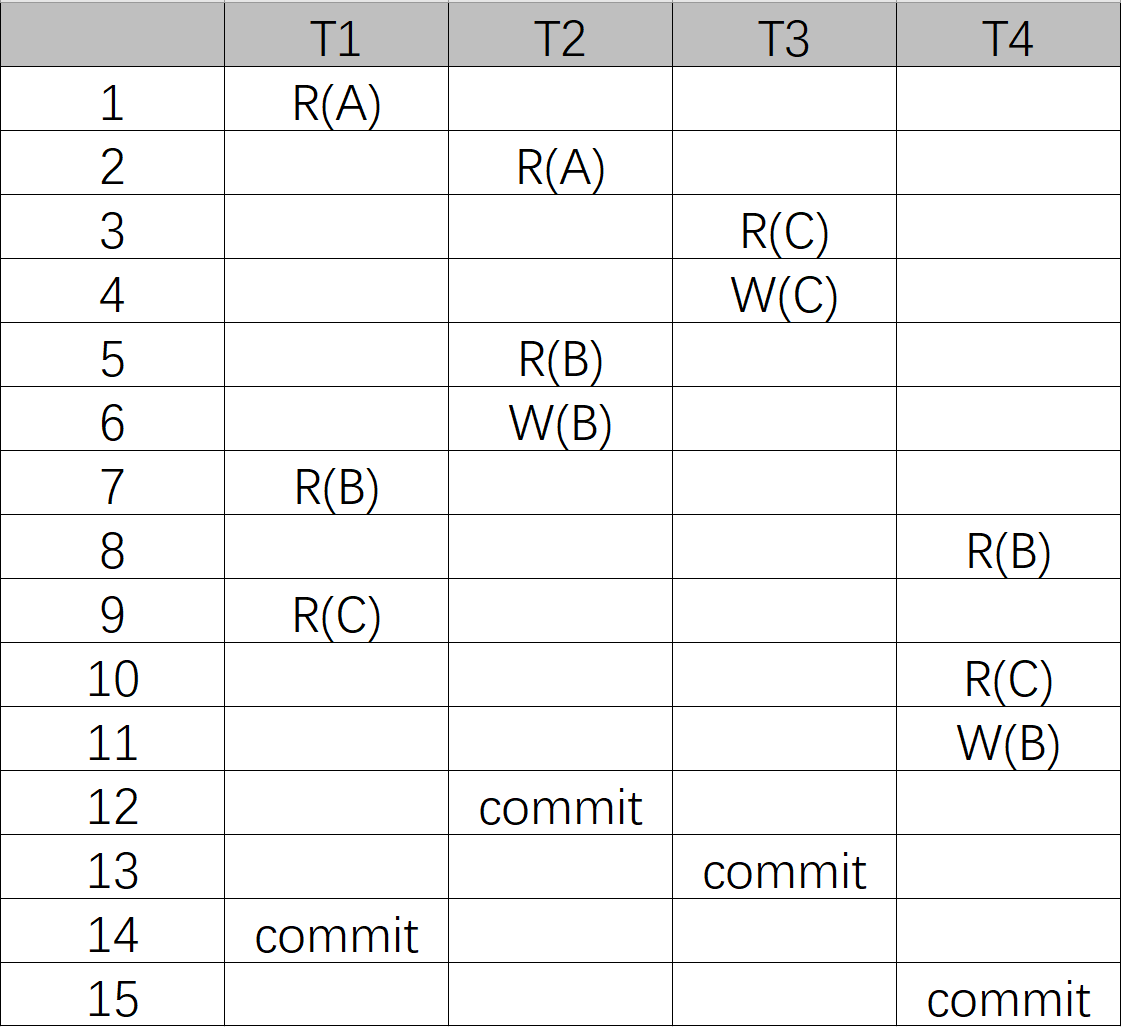
\includegraphics[scale=0.35]{transaction}
	      \end{center}
	      \begin{itemize}
		      \item[(a)] \textbf{[3 points]} Please draw the conflict dependency graph of the above schedule?\\
		            \begin{solution}
			            \begin{center}
				            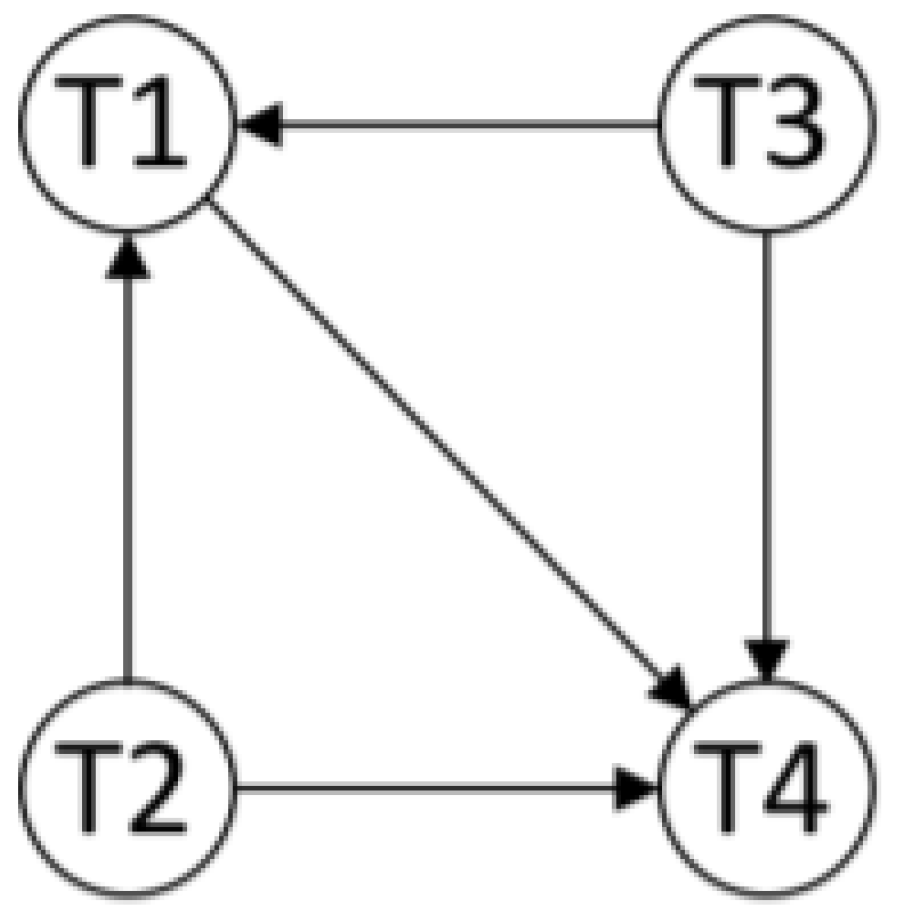
\includegraphics[scale=0.15]{xact_sol_1}
			            \end{center}
		            \end{solution}

		      \item[(b)] \textbf{[3 points]} Which of the following schedules below are conflict equivalent to the schedule above?\\
		            A. T3, T1, T2, T4\\
		            B. T2, T3, T1, T4\\
		            C. T4, T3, T1, T2\\
		            D. T1, T2, T3, T4\\
		            E. T3, T2, T1, T4
		            \begin{solution}
			            B, E.\\
			            Just by doing a topological sort, we know that T4 has to be last and T1 has to be
			            second to last. Whether T2 or T3 comes first is irrelevant since they have no incoming edges,
			            so we have 2 possible conflict equivalent schedules.
		            \end{solution}

		      \item[(c)] \textbf{[3 points]} Mark all the correct choices. \\
		            A. In Strict 2PL, we can give up locks after aborting but before rollback
		            is complete. \\
		            B. Schedules that are conflict serializable can not produce a cyclic
		            dependency graph. \\
		            C. 2PL does not promise conflict serializability. \\
		            D. Strict Two Phase Locking ensures that we do not have deadlocks.

		            \begin{solution}
			            B.
			            \begin{itemize}
				            \item A is false. For A, you must wait until rollback is
				                  complete before giving up locks.
				            \item B is correct. For B, 2PL enforces conflict serializability
				                  but may not allow all conflict serializable schedules (e.g. W1(X),
				                  R2(X), W1(Y), R2(Y) is impossible under 2PL).
				            \item C is false.
				            \item D is false. For D. Strict 2PL does not help us avoid
				                  deadlocks: if T1 wants X(A), X(B), and T2 wants X(B), X(A), we can
				                  get into a deadlock if T1 acquires X(A) and T2 acquires X(B).
			            \end{itemize}
		            \end{solution}

	      \end{itemize}

	\item \textbf{[4 points]} \textbf{Lock Manager} \\
	      Given the database system shown below:
	      \begin{figure}[ht]
		      \centering
		      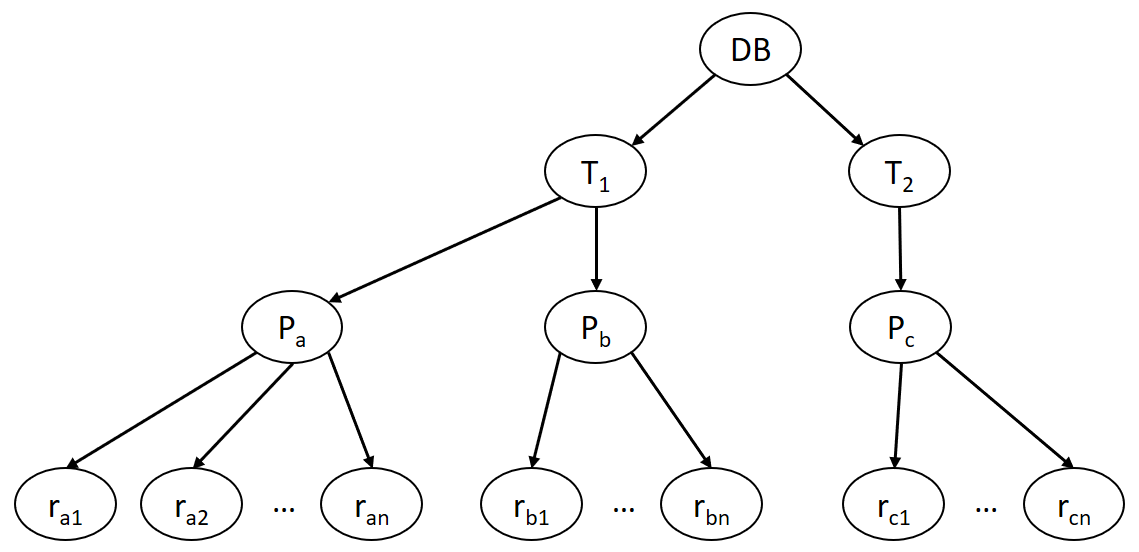
\includegraphics[width=0.7\linewidth]{lock_mode}
	      \end{figure}
	      \begin{itemize}
		      \item[(a)] Which lock modes (including IS, IX, or SIX) on which resources are necessary to read $P_a$?
		      \item[(b)] Which lock modes (including IS, IX, or SIX) held by other transactions on $P_a$ would prevent us from modifying $r_{a1}$?
	      \end{itemize}
	      \begin{solution}
		      \begin{itemize}
			      \item[(a)] We would need the IS lock mode on DB and T1, and the S lock mode on $P_a$. This allows us
			            to read from $P_a$ while restricting other transactions as little as possible.
			      \item[(b)] S, SIX, and X lock modes held by other transactions on $P_a$ would prevent us from holding
			            an X lock on $r_{a1}$, which is necessary to modify $r_{a1}$. IX and IS locks would not prevent us, as
			            the actual X or S locks held by other transactions are not necessarily on $r_{a1}$.
		      \end{itemize}
	      \end{solution}
\end{enumerate}



\newpage
\section{Logging and Recovery \textbf{[20 points]}}

\begin{enumerate}
	\item \textbf{[4 points]} \textbf{ARIES Algorithm} \\
	      Select all the true statements: \\
	      A. Write Ahead Logging describes a protocol where updated pages must be written to disk before a crash. \\
	      B. During a transaction abort, we undo all data updates made by the transaction. \\
	      C. In ARIES, UPDATE log records contain no information of the previous state of the page. \\
	      D. The recovery manager is responsible for Atomicity and Consistency, as defined by the ACID acronym.
	      \begin{solution}
		      B
	      \end{solution}

		  \item \textbf{[5 points]} \textbf{General Logging and Recovery.} \\
	      Mark the boxes for all true statement(s):
	      \begin{itemize}
		      \item[(a)] Schedules produced by two phase locking are guaranteed to prevent cascading aborts.
		            \begin{solution}
			            F: Strict 2PL is needed to guarantee this.
		            \end{solution}
		      \item[(b)] Strict two phase locking is both necessary and sufficient to guarantee conflict serializability.
		            \begin{solution}
			            F: Sufficient but not necessary.
		            \end{solution}
		      \item[(c)] In a system that uses strict two-phase locking, if a transaction aborts, it releases all of its locks as soon as rollback is complete.
		            \begin{solution}
			            T.
		            \end{solution}
		      \item[(d)] In a system that uses strict two-phase locking, a transaction that only performs reads can never enter a deadlock cycle.
		            \begin{solution}
			            F.
		            \end{solution}
		      \item[(e)] When aborting a transaction, it is necessary to modify pages on disk.
		            \begin{solution}
			            T. steal policy.
		            \end{solution}
		      \item[(f)] During recovery, the ARIES protocol redo aborted transactions.
		            \begin{solution}
			            T.
		            \end{solution}
		      \item[(g)] When a transaction commits, any modified buffer pages must be written to durable storage.
		            \begin{solution}
			            F: no force policy.
		            \end{solution}
		      \item[(h)] In ARIES recovery, after the analysis phase, the recLSN of each page in the dirty page table must be larger than the pageLSN of the corresponding page.
		            \begin{solution}
			            F: The page could have been updated and flushed from the buffer pool between the last
			            checkpoint and time of crash. The flushed page would have a pageLSN from its most recent update, which is after the recLSN in the checkpoint.
		            \end{solution}
		      \item[(i)] If PageLSN is greater than the max LSN flushed so far (flushedLSN), we can safely write this page to disk.
		            \begin{solution}
			            T: WAL requires that.
		            \end{solution}
		      \item[(j)] Write-Ahead Logging (WAL) guarantees that a transactions log records are flushed to disk before the transaction commit.
		            \begin{solution}
			            T.
		            \end{solution}
	      \end{itemize}

	\item \textbf{[8 points]} \textbf{Recovery.} \\
	      Your database server has just crashed due to a power outage.
	      You boot it back up, find the following log and checkpoint information on disk,
	      and begin the recovery process. Assume we use a STEAL/NO FORCE recovery policy.
	      \begin{figure}[h]
		      \centering
		      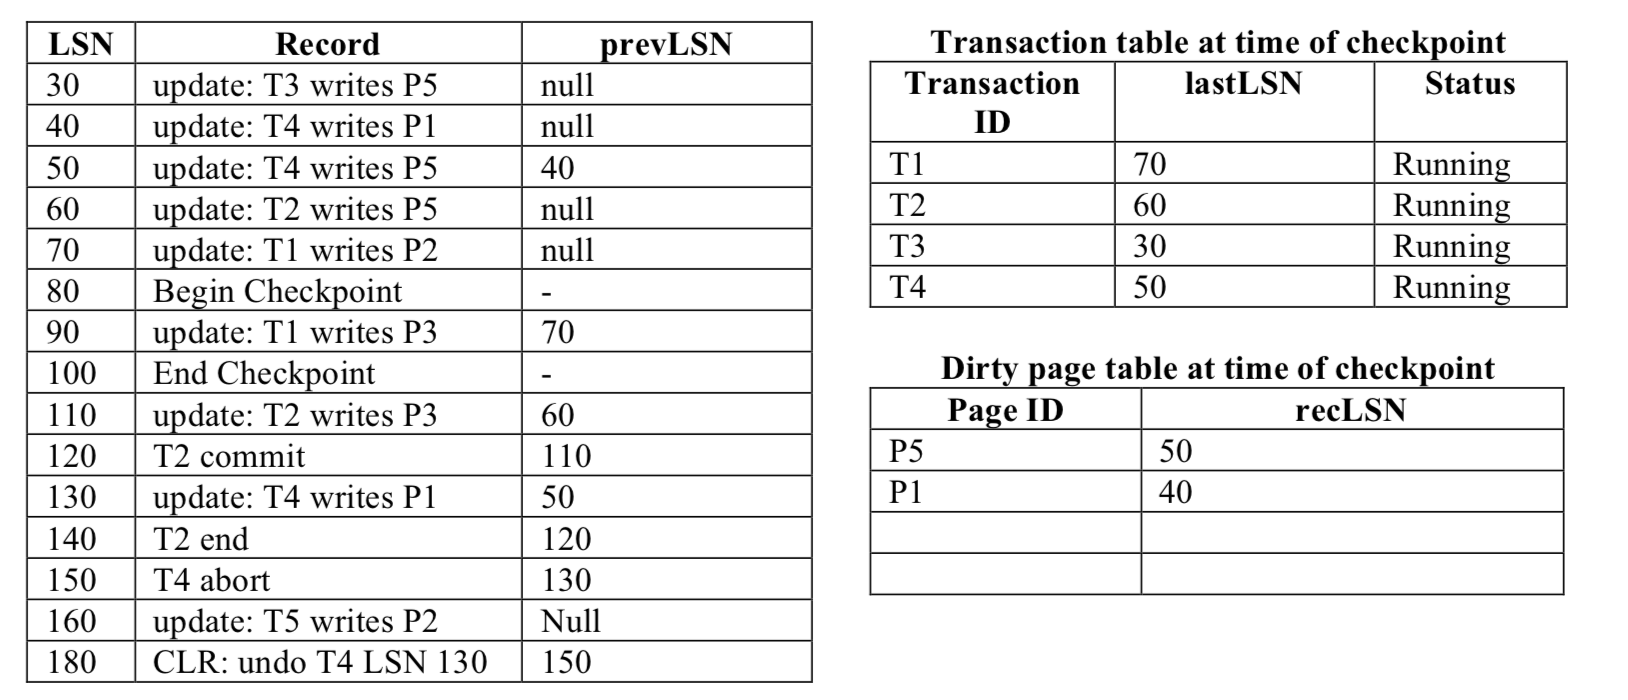
\includegraphics[width=\linewidth]{recovery}
		      %	\caption{Logging and recovery}
		      \label{fig:recovery}
	      \end{figure}
	      \begin{itemize}
		      \item[(a)] \textbf{[2 points]}
		            At the end of the Analysis phase, what transactions will be in the transaction table,
		            and with what lastLSN and Status values?
		            \begin{solution}
			            \begin{center}
				            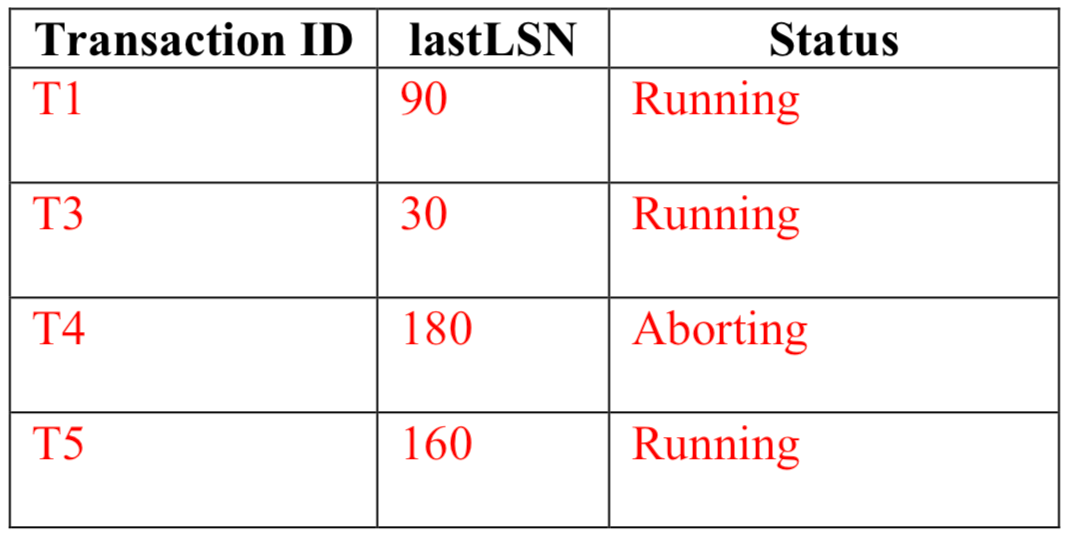
\includegraphics[width=.6\linewidth]{Xact_sol.png}
			            \end{center}
		            \end{solution}
		            We also accept the answer by moving the status of transactions in the above table from ``Running'' to ``Aborting''.
		      \item[(b)] \textbf{[2 points]}
		            At the end of the Analysis phase, what pages will be in the dirty page table, and with what recLSN values?
		            \begin{solution}
			            \begin{center}
				            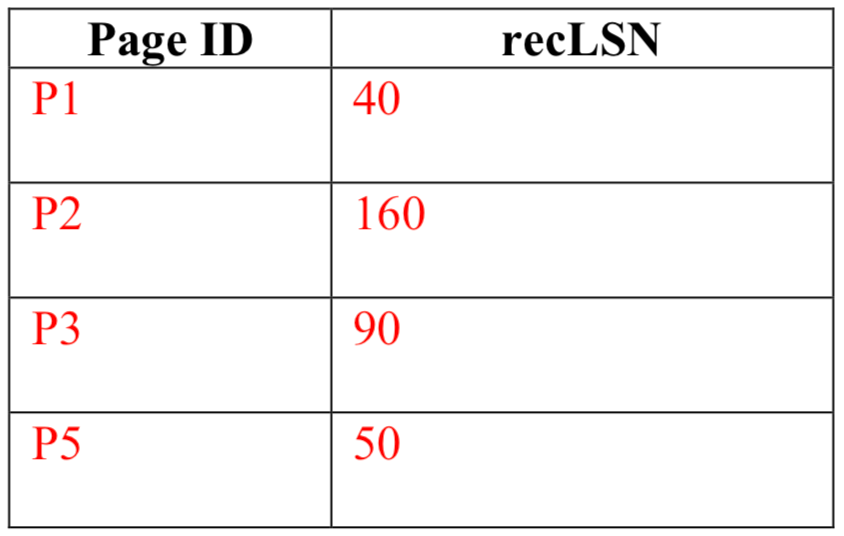
\includegraphics[width=.45\linewidth]{DPT_sol.png}
			            \end{center}
		            \end{solution}
	      \end{itemize}

\end{enumerate}




\newpage
\section{ER Modeling and Functional Dependencies \textbf{[20 points]}}

\begin{enumerate}

	\item \textbf{[4 points]} \textbf{ER Modeling} \\
	      In this question, we will choose to model elements of a baseball league using ER-Diagrams. We have 4 entities:
	      supporters, teams, players, contract and agents. Refer to the diagram below for the following question.
	      \begin{figure}[ht]
		      \centering
		      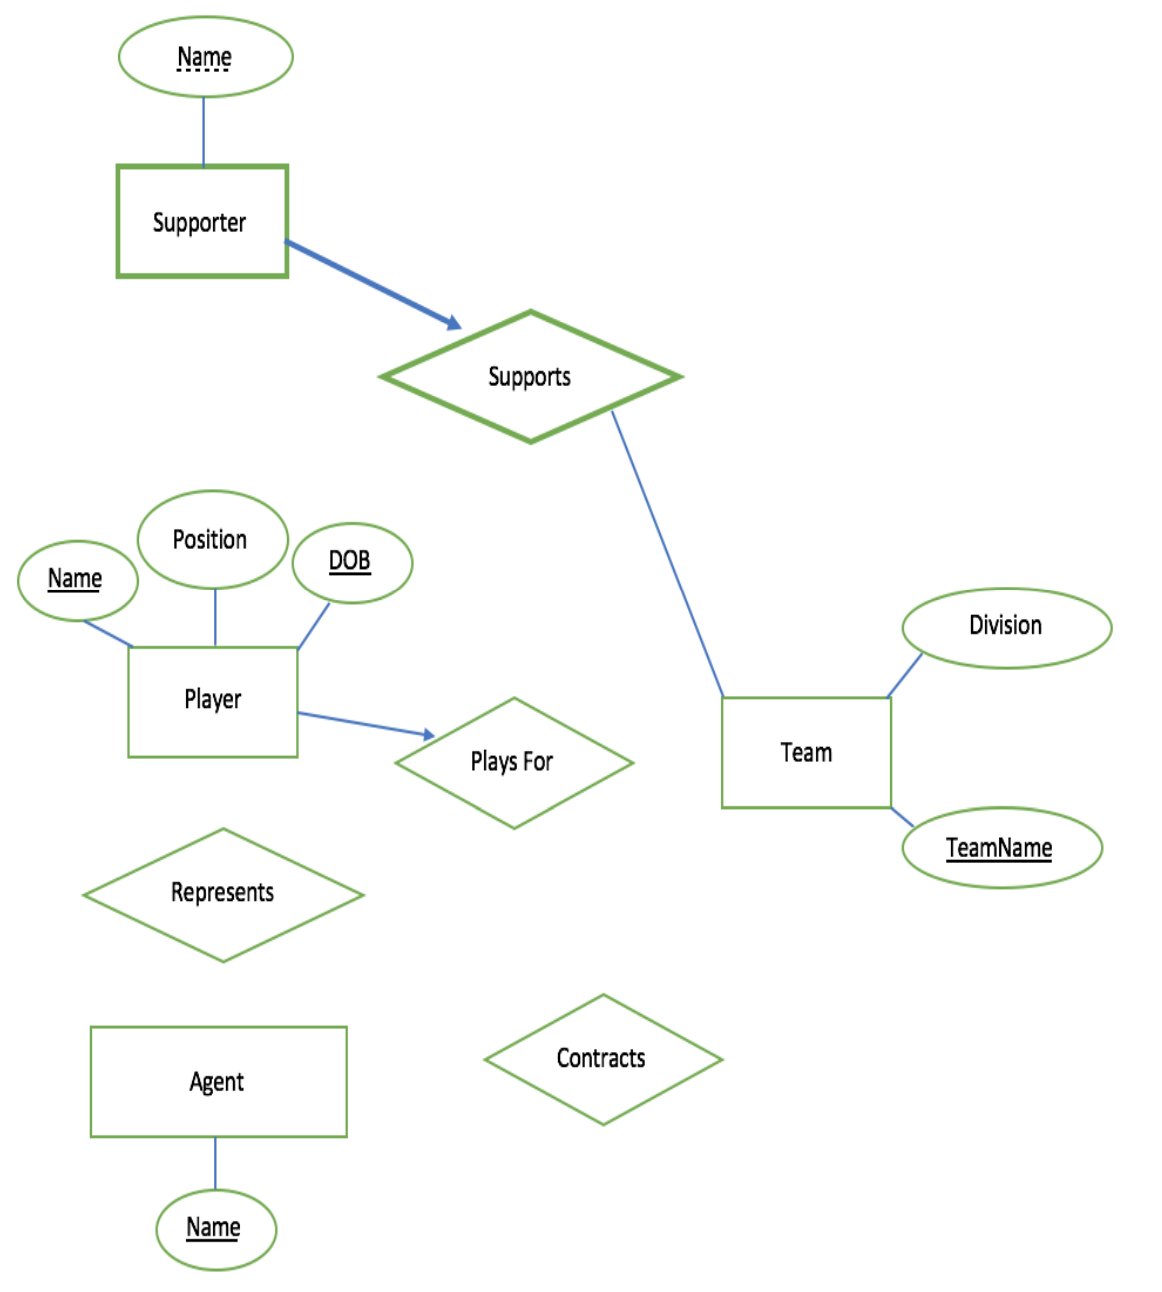
\includegraphics[width=0.7\linewidth]{pro2}
	      \end{figure}

	      \begin{enumerate}
		      \item There are some elements of the ER-diagram are missing, fill them in so that the ER-diagram satisfies the following constraints.

		            \begin{itemize}
			            \item Each team must have at least one players on its roster.
			            \item Each player must have exactly one agent to represent him/her.
			            \item Each agent can sign as many contracts as he or she wants to, or none at all.
			            \item Each player can have at most one contract.
			            \item A team has at least one contract.
			            \item Relation \textbf{Represents} involves entities \textbf{Player} and \textbf{Agent}; relation \textbf{Contracts} involves
			                  entities \textbf{Player}, \textbf{Agent} and \textbf{Team}; relation \textbf{Plays For} involves entities \textbf{Team} and \textbf{Player}
		            \end{itemize}

		            Hint: you should add 6 edges in total.

		            \begin{solution}

			            %\begin{figure}[ht]
			            \centering
			            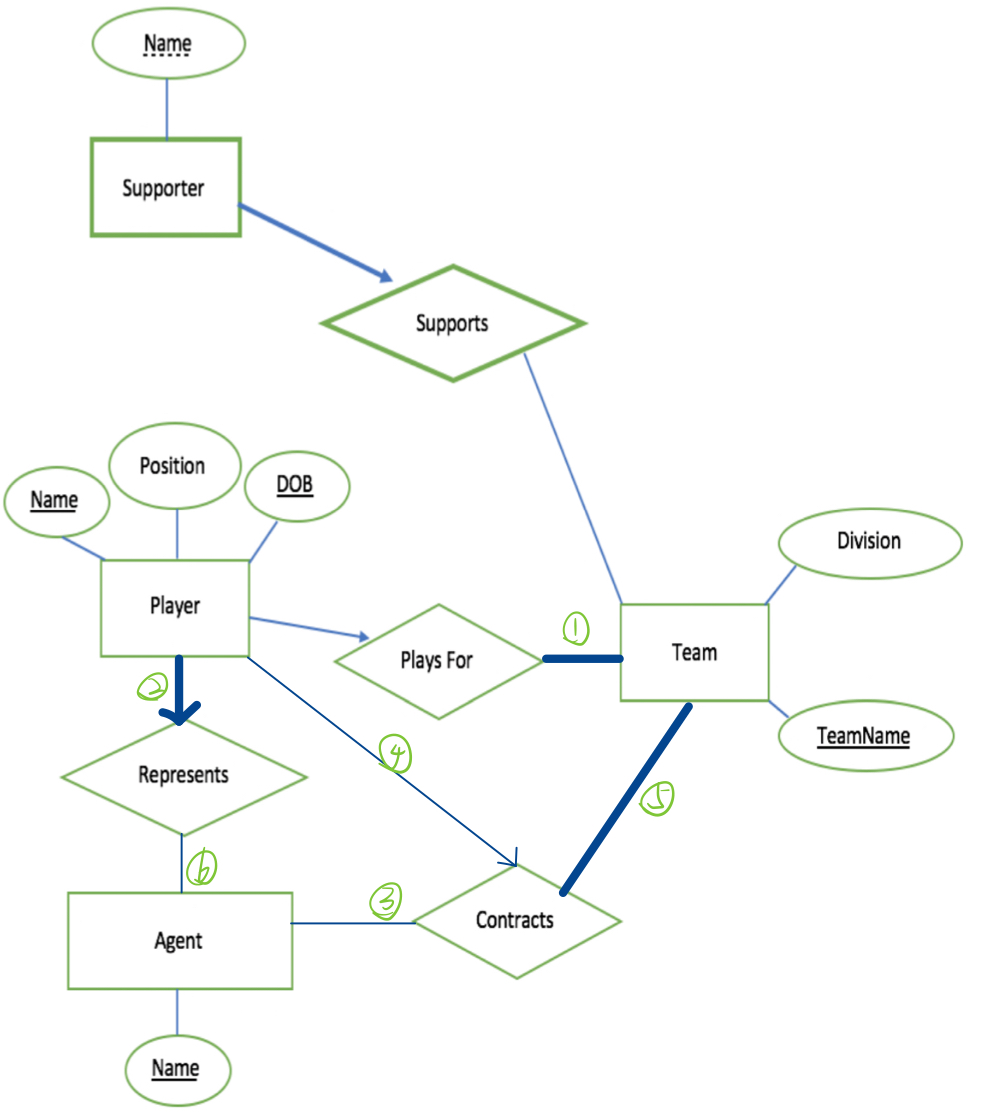
\includegraphics[width=0.7\linewidth]{pro2_1}
			            %\end{figure}

		            \end{solution}

		      \item As \textbf{Supporter} is a weak entity that must have unique and total participation in the \textbf{Supports} relation,
		            its primary key is determined by which attribute(s) in the ER-diagram? \\
		            A. Name \\
		            B. TeamName \\
		            C. Name, TeamName \\
		            D. None of them

		            \begin{solution}
			            C
		            \end{solution}
	      \end{enumerate}



	\item \textbf{[4 points]} \textbf{FD Properties} \\
	      Select all the FD's that follow from Armstrong's Axiom.
	      Select all true statement(s): \\
	      A. if X → Y and Z → W, then XZ → YW \\
	      B. if XZ → YZ, then X → Y \\
	      C. if X → YZ, then X → Y and X → Z \\
	      D. if X → Y and WY → Z, then WX → Z \\
	      E. if X → Y and W → Y, then X → W \\
	      \begin{solution}
		      A, C, D
	      \end{solution}

	\item \textbf{[4 points]} \textbf{FD Example} \\
	      We have a relation R(A, B, C, D, E). We are told that the set of functional dependencies is
	      F = {E → BC, A → B, C → D, AD → C}.
	      \begin{itemize}
		      \item[(a)] What are A+, C+ and E+
		      \item[(b)] Is the attribute set ACE the superkey for relation R?
		      \item[(c)] Is relation R already in Boyce-Codd Normal Form (BCNF)?
	      \end{itemize}
	      \begin{solution}
		      \begin{itemize}
			      \item[(a)] A+: AB, C+: CD, E+: BCDE.
			      \item[(b)] Yes. ACD+: ABCDE.
			      \item[(c)] No. None of the the FDs are a superkey of R and none of them are trivial FDs.
		      \end{itemize}
	      \end{solution}

	\item \textbf{[4 points]} \textbf{Normalization and Decomposition} \\
	      Decompose ABCDEFGH into Boyce-Codd Normal Form (BCNF) in the order of the following FDs:
	      G → H; EF → B; EA → C; FH → D.
	      \begin{solution}
		      At step 1, we get ABCDEFG and GH. \\
		      At step 2, we get ACDEFG and EFB and GH. \\
		      At step 3, we get ADEFG and EAC and EFB and GH.
	      \end{solution}


\end{enumerate}



\newpage
\section{Parallel Query Processing \textbf{[20 points]}}

\begin{enumerate}

	\item \textbf{[4 points]} \textbf{Partition} \\
	      Assume that we have 5 machines and a 1000 page \textbf{students(sid, name, gpa)} table. Initially,
	      all of the pages start on one machine. Assume pages are 1KB.
	      \begin{itemize}
		      \item[(a)] How much network cost does it take to round-robin partition the table?
		      \item[(b)] How many IOs will it take to execute the following query:
		            \begin{lstlisting} 
  SELECT *
  FROM students
  WHERE name = 'John'
\end{lstlisting}
		      \item[(c)] Suppose that instead of round robin partitioning the table, we hash partitioned it on the name
		            column instead, How many IOs would the query from (b) take?
		            (Assume that all records with value 'John' can fit on one machine.)
		      \item[(d)] Assume that an IO takes 1ms and the network cost is negligible. How long will the query in part
		            2 take if the data is round-robin partitioned and if the data is hash partitioned on the name column?
		            (For simplicity, assume that each machine spends the same amount of time on scanning.)
	      \end{itemize}
	      \begin{solution}
		      \begin{itemize}
			      \item[(a)] 800 KB. \\
			            In round robin partitioning the data is distributed completely evenly. This means that the ma-
			            chine the data starts on will be assigned 1/5 of the pages. This means that 4/5 of the the pages
			            will need to move to different machines, so the answer is: 4/5 * 1000 * 1 = 800 KB.
			      \item[(b)] 1000 IOs. \\
			            When the data is round robin partitioned we have no idea what machine(s) the records we
			            need will be on. This means we will have to do full scans on all of the machines so we will have to
			            do a total of 1000 IOs.
			      \item[(c)] 200 IOs. \\
			            When the data is hash partitioned on the name column, we know exactly what machine to
			            go to for this query (we can calculate the hash value of 'John' and find out what machine is
			            assigned that hash value). This means we will only have to a full scan over 1 machine for a total
			            of 200 IOs. Of course, this assumes all records with value 'John' can fit on one machine.
			      \item[(d)] 200ms. \\
			            Under both partitioning schemes it will take 200ms. Each machine will take the same amount
			            of time to do a full scan, and all machines can be run at the same time so for runtime it doesn't
			            matter how many machines we need to query.
		      \end{itemize}
	      \end{solution}

	\item \textbf{[4 points]} \textbf{Parallel Algorithm} \\
	      Assume that we have a 100 page table R that we will join with a 400 page table S.
	      All the pages start on machine 1, and there are 4 machines in total with 30 buffer pages each.
	      \begin{itemize}
		      \item[(a)] How many passes are needed to do a parallel unoptimized SMJ on the data? For
		            this question a pass is defined as a full pass over either table (so if we have to do 1 pass over R and 1 pass
		            over S it is 2 total passes).
		      \item[(b)] How many passes are needed to a parallel Grace Hash Join on the data?
		      \item[(c)] We want to calculate the max in parallel using hierarchical aggregation. What value should
		            each machine calculate and what should the coordinator do with those values?
	      \end{itemize}
	      \begin{solution}
		      \begin{itemize}
			      \item[(a)] 7 passes.\\
			            2 passes to partition the data (1 for each table). Each machine will then have 25 pages for R
			            and 100 pages for S. R can be sorted in 1 pass but S requires 2 passes. Then it will take 2 passes
			            to merge the tables together (1 for each table). This gives us a total of 2 (partition) + 1 (sort R)
			            + 2 (sort S) + 2 (merge relations) = 7 passes.
			      \item[(b)] 4 passes. \\
			            We will need 2 passes to partition the data across the four machines and each machine
			            will have 25 pages for R and 100 for S. We don't need any partitioning passes because R fits in
			            memory on every machine, so we only need to do build and probe, which will take 2 passes (1 for
			            each table). This gives us a total of 4 passes.
			      \item[(c)] Each machine should calculate the max and the coordinator will take the max of those maxes.
		      \end{itemize}
	      \end{solution}

\end{enumerate}





\newpage
\section{Distributed Transactions and NoSQL \textbf{[20 points]}}

\begin{enumerate}
	\item \textbf{[4 points]} \textbf{2-Phase Commit} \\
	      True or False: \\
	      \begin{itemize}
		      \item[(a)] If we are recovering and see a PREPARE record, it means we must have sent out a YES vote.
		      \item[(b)] If the coordinator is recovering and sees a COMMIT record, we can locally commit and end the process there.
		      \item[(c)] Suppose a participant receives a prepare message for a transaction and replies VOTE-YES.
		            Suppose that they were running a wound-wait deadlock avoidance policy, and a transaction
		            comes in with higher priority. The new transaction will abort the prepared transaction.
	      \end{itemize}
	      \begin{solution}
		      \begin{itemize}
			      \item[(a)] False. \\
			            We could have crashed between logging PREPARE and sending VOTE-YES.
			      \item[(b)] False. \\
			            There is no guarantee that all participants received a COMMIT record, so we must rerun phase 2 first.
			      \item[(c)] False. \\
			            Transactions that are prepared must be ready to commit if the coordinator tells them
			            to, so they cannot be aborted by anyone other than the coordinator.
		      \end{itemize}
	      \end{solution}

	\item \textbf{[4 points]} \textbf{OLTP and OLAP} \\
	      Are the following workloads better characterized as Online Transaction Processing (OLTP)
	      or Online Analytical Processing (OLAP)?
	      \begin{itemize}
		      \item[(a)] Placing orders and buying items in an online marketplace
		      \item[(b)] Analyzing trends in purchasing habits in an online marketplace
	      \end{itemize}
	      \begin{solution}
		      \begin{itemize}
			      \item[(a)] OLTP. \\
			            OLTP workloads involve high numbers of transactions executed by many different users.
			            Queries in these workloads involve simple lookups more often than complex
			            joins. In this case, when a user buys an item, the site might perform actions like looking
			            up the item and updating its quantity, recording a new purchase, etc.
			      \item[(b)] OLAP.\\
			            OLAP workloads involve read-only queries and typically include lots of joins
			            and aggregations. Often, workloads executed for analysis and decision making are OLAP
			            workloads.
		      \end{itemize}
	      \end{solution}


		  	\item \textbf{[4 points]} \textbf{NoSQL} \\
		  	True or False:
	      \begin{itemize}
		      \item[(a)] As methods for scaling dataset, partitioning is effective for write-heavy workloads, and replicaction is effective for read-heavy workloads.
		      \item[(b)] Partitioning and replication are often used together in real systems to leverage the performance
			  benefits and to make the system more fault-tolerant.
		      \item[(c)] The consistency in the distributed systems is the same concept with the consistency found in ACID (Transactions).
		      \item[(d)] JSON and XML are referred as semi-structured data formats, and can express complex data structures, which may be arranged into nested structures.
		      \item[(e)] JSON is self-describing, and it is designed for efficient storage and retrieval from disk.
	      \end{itemize}
	      \begin{solution}
		      \begin{itemize}
			      \item[(a)] True.
			      \item[(b)] True.
			      \item[(c)] False.
			      \item[(d)] True.
			      \item[(e)] False.
		      \end{itemize}
	      \end{solution}


		  \iffalse
		  \item \textbf{[4 points]} \textbf{JSON Semantic} \\
		  A JSON document can be represented by a semantic tree, as shown in the following figure.
		  Draw the 
		  \fi

\end{enumerate}


\newpage
\section{MapReduce and Spark \textbf{[20 points]}}

\begin{enumerate}

	\item \textbf{[4 points]} \textbf{Basics} \\
	      True or False:
	      \begin{itemize}
		      \item[(a)] In MapReduce, the Map phase applies a function in parallel to every element of a set of data, and the Reduce phase combines the
		            results of the Map phase into the desired data output.
		      \item[(b)] In Distributed File System (DFS), a file system in which large files are partitioned into smaller files,
		            and then distributed and replicated several times on different nodes for fault tolerance.
		      \item[(c)] Both the Map and Reduce phases can be split among dfferent
		            workers on different machines, with workers performing independent tasks in parallel.
		      \item[(d)] Since the Reduce phase must wait until the entire Map phase completes, we must restart the entire Map phase if one map task
		            fails.
		      \item[(e)] Resilient Distributed Datasets (RDDs) are not written to disk in intermediate steps but are rather stored in main memory.
		      \item[(f)] Similar with MapReduce, Spark needs to write intermediate results to disk.
	      \end{itemize}
	      \begin{solution}
		      \begin{itemize}
			      \item[(a)] True.
			      \item[(b)] True.
			      \item[(c)] True.
			      \item[(d)] False.
			      \item[(e)] True.
			      \item[(f)] False.
		      \end{itemize}
	      \end{solution}


	\item \textbf{[4 points]} \textbf{MapReduce} \\
	      \begin{itemize}
		      \item[(a)]  Fig.~\ref{mr1} shows a relation $R(A)$ with the MapReduce implementation of the Selection operator $\sigma_{A=123}(R)$.
		            \begin{figure}[H]
			            \centering
			            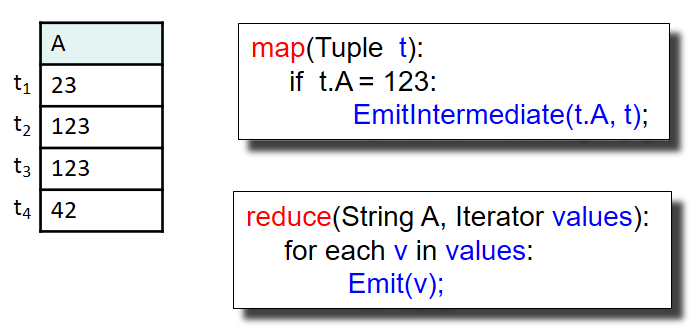
\includegraphics[width=0.5\linewidth]{mr_selection}
			            \caption{Selection}
			            \label{mr1}
		            \end{figure}
		            \begin{itemize}
			            \item[(1)] What is the output of the Map function?
			            \item[(2)] What is the output of the Reduce function?
		            \end{itemize}
		      \item[(b)]  Fig.~\ref{mr2} shows a relation $R(A,B)$ with the MapReduce implementation of the Group-By operator $\gamma_{A=123,\text{SUM} (B)}(R)$.
		            \begin{figure}[H]
			            \centering
			            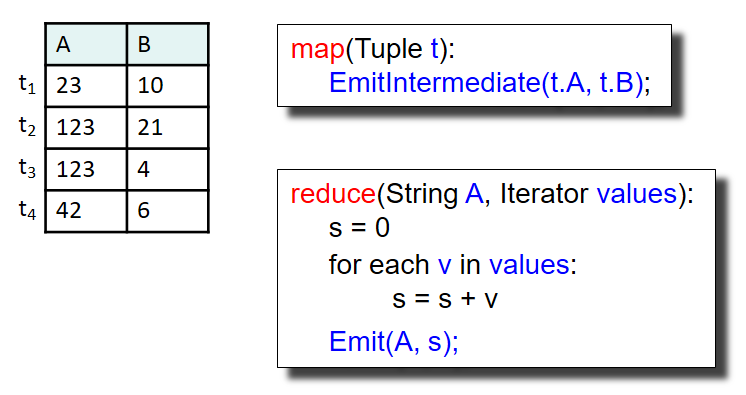
\includegraphics[width=0.5\linewidth]{mr_group}
			            \caption{Group-By}
			            \label{mr2}
		            \end{figure}
		            \begin{itemize}
			            \item[(1)] What is the output of the Map function?
			            \item[(2)] What is the output of the Reduce function?
		            \end{itemize}
		      \item[(c)]  Fig.~\ref{mr3} shows two relations $R(A,B)$ and $S(C,D)$ with the MapReduce implementation of the Hash-Join operator $R(A,B) \bowtie_{B=C} S(C,D)$.
		            \begin{figure}[H]
			            \centering
			            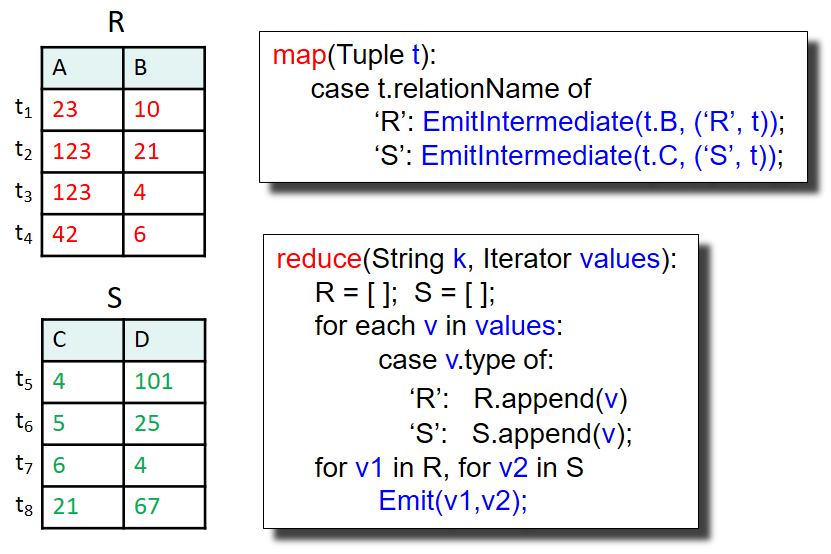
\includegraphics[width=0.55\linewidth]{mr_join}
			            \caption{Hash-Join}
			            \label{mr3}
		            \end{figure}
		            \begin{itemize}
			            \item[(1)] What is the output of the Map function?
			            \item[(2)] What is the output of the Reduce function?
		            \end{itemize}
	      \end{itemize}
	      \begin{solution}
		      \begin{itemize}
			      \item[(a)] (1) $(123,[t_2,t_3])$ \\ (2) $(t_2,t_3)$. 
			      \item[(b)] (1) $(23,[t_1])$, $(42,[t_4])$, $(123,[t_2,t_3])$ \\ (2) $(23,10)$, $(42,6)$, $(123,25)$. 
			      \item[(c)] 		            
				  \begin{figure}[H]
			            \centering
			            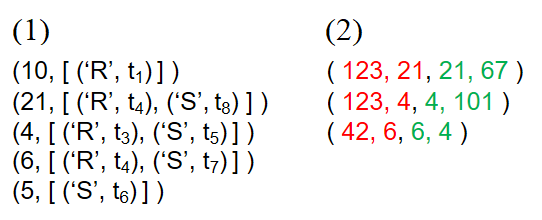
\includegraphics[width=0.45\linewidth]{mr_sol}
		            \end{figure}
		      \end{itemize}
	      \end{solution}


\end{enumerate}





\newpage
\section{Data Mining and Machine Learning \textbf{[20 points]}}

\begin{enumerate}

\item \textbf{[4 points]} \textbf{General Data Mining and Machine Learning.} \\
	      Mark the boxes for all true statement(s):
	      \begin{itemize}
		      \item[(a)] In multi-dimensional data model, it contains one fact table and multiple dimension tables.
		            \begin{solution}
			            True.
		            \end{solution}
		      \item[(b)] The order of the basic KDD (Knowledge Discovery in Database) process is Data Selection, Data Cleaning, Evaluation, Data Mining \& ML.
		            \begin{solution}
			            False: Data Mining comes before Evaluation.
		            \end{solution}
		      \item[(c)] In supervised machine learning labeled data is used to train a model.
		            \begin{solution}
			            True: The labeled data is the “supervision” in the name.
		            \end{solution}
		      \item[(d)] Classification models would be a good candidate when trying to predict the total
		            amount of time a user spends browsing a page.
		            \begin{solution}
			            False: Classification produces a discrete label (like “True/False”);
			            to get a numeric value like an amount of time you might want to use regression.
		            \end{solution}
		      \item[(e)] The ultimate goal in machine learning is to find a model that best fits the training data.
		            \begin{solution}
			            False: Fitting the training data is a means to the end goal of predicting unknown
			            information.  As we learned, you can overfit the training data if you make that your
			            ultimate goal.
		            \end{solution}
		      \item[(f)] The $k$-means algorithm is guaranteed to converge to the global optimum.
		            \begin{solution}
			            False: $k$-means can produce a sub-optimal answer,
			            and it sensitive to the initial position of the centers;
			            it does compute what’s called a ``local optimum''.
		            \end{solution}
		      \item[(g)] The bag-of-words model encodes text as a vector.
		            \begin{solution}
			            True.
		            \end{solution}
		      \item[(h)] A common form of feature engineering on continuous data is one-hot-encoding.
		            \begin{solution}
			            False: One-hot encoding is used for capturing the presence of boolean features.
		            \end{solution}
	      \end{itemize}

	\item \textbf{[8 points]} \textbf{K-Means.}
	      \begin{itemize}

		      \item[(a)] \textbf{[2 points]}
		            Which of the following can act as possible termination conditions in $k$-means?
		            (you may mark zero ($\phi$), one or more than one of the choices.)\\
		            A. For a fixed number of iterations.\\
		            B. Assignment of observations to clusters does not change between iterations. Except for cases with a bad local minimum.\\
		            C. Centroids do not change between successive iterations.\\
		            D. Terminate when the objective value falls below a threshold.
		            \begin{solution}
			            A, B, C, D.\\
			            All four conditions can be used as possible termination condition in K-Means clustering:

			            This condition limits the runtime of the clustering algorithm, but in some cases the quality of the clustering will be poor because of an insufficient number of iterations.
			            Except for cases with a bad local minimum, this produces a good clustering, but runtimes may be unacceptably long.
			            This also ensures that the algorithm has converged at the minima.
			            Terminate when the objective value falls below a threshold. This criterion ensures that the clustering is of a desired quality after termination. 
						Practically, it’s a good practice to combine it with a bound on the number of iterations to guarantee termination.
		            \end{solution}


		      \item[(b)] \textbf{[2 points]}
		            In which of the following cases will $k$-means clustering fail to give good results?
		            (you may mark zero ($\phi$), one or more than one of the choices.)\\
		            A. Data points with outliers.\\
		            B. Data points with different densities.\\
		            C. Data points with round shapes.\\
		            D. Data points with non-convex shapes.
		            \begin{solution}
			            A, B, D.\\
			            K-Means clustering algorithm fails to give good results when the data contains outliers, the density spread of data points across the data space is different and the data points follow non-convex shapes.
		            \end{solution}

		      \item[(c)] \textbf{[2 points]}
		            The following is a set of one-dimensional points: $\{-4, 0, 1, 2, 3, 5, 7, 10, 13, 22\}$, perform two iterations of $k$-means on these points using the two initial centroids 1 and 7.
		            \begin{itemize}
			            \item[1)] What are the two new centroids after the first iteration?
			            \item[2)] What are the two new centroids after the second iteration?
		            \end{itemize}
		            \begin{solution}
			            first iteration: 2/5; 57/5\\
			            second iteration: 7/6; 13
		            \end{solution}
	      \end{itemize}



	\item \textbf{[4 points]} \textbf{Linear Regression} \\
	      Given $n$ independent and identically distributed (i.i.d.) training samples
	      $\{(x_1, y_1), (x_2, y_2), ... , (x_n, y_n)\}$, with the $i$-th sample $x_i, y_i \in \mathbb{R}$, $i=1,2,...,n$.
	      Consider the linear model:
	      \begin{equation}
		      y = x\theta + \epsilon \quad \epsilon\sim\mathcal{N}(0,\,\sigma^{2}),
	      \end{equation}
	      where $\mathcal{N}(0,\,\sigma^{2})$ denotes the Guassian distribution with mean 0 and variance $\sigma^2$.
	      Assume that the training data has been centralized, such that the intercept can be ignored in the above linear model.
	      Obviously, the probability density function of $y$ conditioned on $x$ and $\theta$ follows the Gaussian distribution $\mathcal{N}(x\theta,\sigma)$,
	      which is defined by
	      \begin{equation}
		      p(y|x,\theta) = \frac{1}{\sqrt{2\pi\sigma^2}}\exp(-\frac{1}{2\sigma^2}(y-x\theta)^2).
	      \end{equation}
	      The model parameter $\theta$ can be estimated based on Maximum Likelihood Estimation (MLE), which aims to maximize the likelihood function:
	      \begin{align}
		      L(\theta) & = \prod_{i=1}^n P(x_i,y_i|\theta) \nonumber                                                   \\
		                & = \prod_{i=1}^n P(y_i|\theta, x_i)P(x_i) \nonumber                                            \\
		                & = \prod_{i=1}^n \frac{1}{\sqrt{2\pi}\sigma}\exp(-\frac{(y_i - x_i\theta)^2}{2\sigma^2})P(x_i)
	      \end{align}
	      \begin{itemize}
		      \item[(a)] Show the log-likelihood function $\log L(\theta)$. (The base of the log function is $e$.)
		      \item[(b)] Using MLE to calculate the closed-form solution of $\theta$.
	      \end{itemize}

	      \begin{solution}
		      \begin{itemize}
			      \item[(a)] According to the definition of the likelihood function, we have
			            \begin{align}
				            \log L(\theta) & = \sum_{i=1}^n -\frac{1}{2}\log 2\pi - \log \sigma - \frac{(y_i-x_i\theta)^2}{2\sigma} + \log P(x_i) \nonumber \\
				                           & = -\frac{1}{2\sigma} \sum_{i=1}^n(y_i-x_i\theta)^2 + C,
			            \end{align}
			            where $C$ denotes a constant, and it is irrelevant to $\theta$.
			      \item[(b)]
			            Based on (a), we have
			            \begin{equation}
				            \hat{\theta} = \argmax_{\theta} \log L(\theta) = \argmin \sum_{i=1}^n (y_i-x_i\theta)^2.
			            \end{equation}
			            By seting the derivative of above objective function w.r.t. $\theta$ equal to 0, we have
			            \begin{equation}
				            \theta = \frac{\sum_{i=1}^n x_i y_i}{\sum_{i=1}^n x_i^2}.
			            \end{equation}
		      \end{itemize}
	      \end{solution}

\end{enumerate}




\iffalse
	\item \textbf{[4 points]} \textbf{2-Phase Commit} \\
	Suppose we would like to translate the following data from the relational model to JSON
	in migrating to a NoSQL database like MongoDB. Given that we want to be able to list all
	purchases a user made without performing any joins or aggregations, what will the resulting
	JSON document look like?
	\begin{figure}[ht]
		\centering
		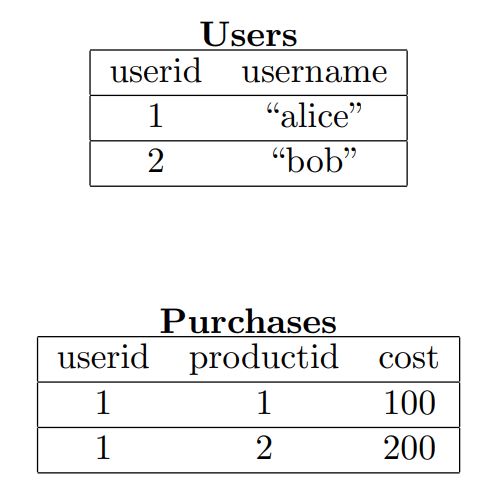
\includegraphics[width=0.3\linewidth]{nosql_json}
	\end{figure}
	\end{enumerate}
\fi


\end{document}

